\chapter{Weekly Write-Up}\label{C:us}

\section{Progress}

Main points this week; multi-threading is now working, built some more items to work with sentiment140 API.\\

\subsection{Multi-Threading} I learned how to do multi-threading in ruby, and implemented it! A thread pool of 15 is created. Each thread then sends an http request to fetch the detailed tweet data, allowing retweets, favourites, date/time data to be accessed by the scraper. If a request fails, it is simply discarded in order to not reduce the benefit of parellisation. Multi-threading has increased performance dramatically. In my evaluation, I may make the point that fetching an entire profile as a policy might be too time-consuming to be useful. A good policy input might be to specify the number of tweets required for reputation analysis. 

%INSERT THE IMAGE HERE!!
\begin{figure}[h!]
\centering
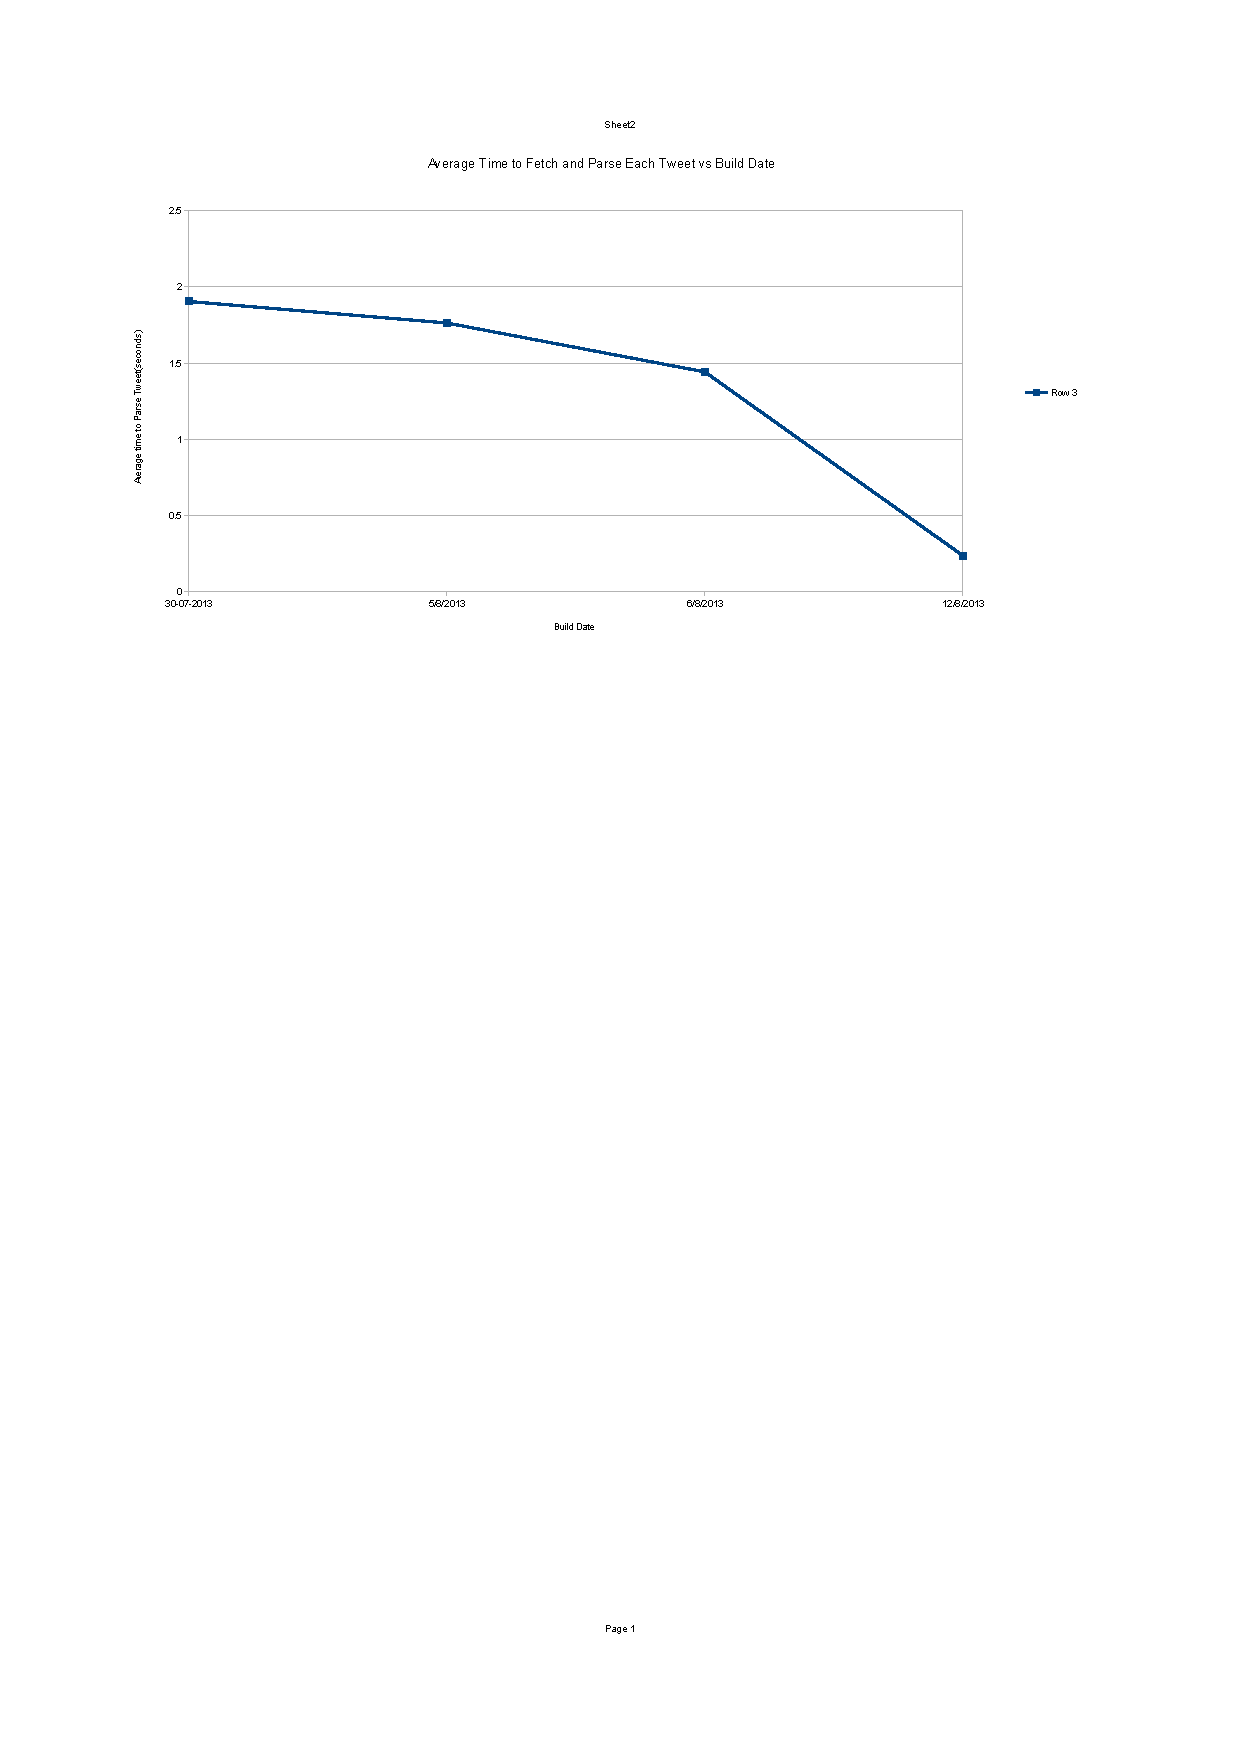
\includegraphics{Images/average_time_to_fetch_parse_tweets_per_build.pdf}
\caption{The Average Time to Fetch and Parse a Tweet, Ordered by Builds}
\end{figure}


\subsection{Sentiment}

I can input my tweets, and retrieve a response positive/neutral/negative. Initial results included, I save these as csv format to import into excel more easily.\\

\subsection{Blockers}

Found the issue causing the correlation between month/overall impact to be incorrect. The graph indeed showed that there was a problem with the data collected. This was in fact from the scraper. Scraper was in fact including tweets NOT posted by the page owner (retweets) and counting these as retweets towards the individual's impact factor. Have fixed this, but did not have enough time to gather sufficient and accurate data for the meeting.\\

\noindent This is not such a massive problem overall - but it will have largely skewed impact results for less popular pages in the past.

\subsection{Targets}

Targets for this week; gather lots more data (accurate) and do the correlation analysis on this. With this more accurate data, look at how sentiments - positive and negative, correlate with the impact formula calculation. Case studies; contraversial individuals and the like. 
